\section{Confiabilidade dos Modelos de Aprendizado de Máquina}
\label{cap:2.4}

Inserir um conjunto específico de dados na entrada de um modelo de aprendizado de máquina, capturar sua resposta e compará-la com a resposta esperada é a forma mais simples de verificação da exatidão da resposta desse modelo. No entanto, um único caso de teste não é estatisticamente válido, por isso, utilizam-se diversos casos, preferencialmente diferentes dos utilizados para treinamento. A média de acertos ($\mu$), definida pela Equação \ref{eq:1}, é pouco empregada de forma isolada na literatura científica, pois não informa muito sobre que tipos de acertos e erros foram performados.

\begin{equation}
    \label{eq:1}
    \mu = \frac{acertos}{total}
\end{equation}

Aqui é importante definir que os modelos de aprendizado de máquina podem retornar respostas complexas. Contudo, para facilitar as explicações desta seção, consideramos modelos cujas respostas sejam valores binários. Inclusive, essa é a forma mais comum de respostas que se observam nos trabalhos com codificação de vídeo. Assim exposto, são esperados quatro tipos de respostas de qualquer modelo com decisões binárias: 

\begin{enumerate}[a)]
    \item \textbf{Verdadeiros Positivos} (VP), ou seja, o modelo retorna positivo quando a resposta de fato é positiva;
    
    \item \textbf{Verdadeiros Negativos} (VN), ou seja, o modelo retorna negativo quando a resposta de fato é negativa;
    
    \item \textbf{Falso Negativo} (FN), quando o modelo retorna negativo quando deveria ter retornado positivo;
    
    \item \textbf{Falso Positivo} (FP), quando o modelo retorna positivo quando deveria ter retornado negativo.
\end{enumerate}

É importante ressaltar que, em modelos cuja decisão possue um rótulo não-binário, esses quatro tipos de resposta ainda estão presentes, mas distribuídos em $2^{rotulos}$ subtipos. Nesta tese, não abordamos avaliações dessa complexidade, mas as referências para tal estão disponíveis em \citet{bib:livroKubat}, \citet{bib:livroML} e \citet{bib:livroRaschka}. Segundo essas referências, as quatro respostas de um modelo binário resultam na matriz de confusão (do inglês, \textit{confusion matrix}), representada na Tabela \ref{tab:II}, na qual, na diagonal, estão as respostas corretas e, nas demais células, estão as respostas erradas.

\begin{table}
\begin{center}
\caption{Matriz de confusão das respostas de um modelo de aprendizado de máquina.}
\label{tab:II}
\footnotesize

\begin{tblr}{
    colspec = {c|c|c|c},
    hlines,
    row{even} = {gray9}
}
\hline
\SetCell[c=2,r=2]{}&& \SetCell[c=2]{c}\textbf{Rótulos Preditos} \\
&& \textbf{Positivo} & \textbf{Negativo} \\
\SetCell[r=2]{c}\textbf{Rótulos Esperados} & \textbf{Positivo} & VP & FN \\
 & \textbf{Negativo} & FP & VN \\
\hline
\end{tblr}
\end{center}
\end{table}


Com essa matriz de confusão, é possível estabelecer o desbalanceamento da predição feita pelo modelo. É esperado que, na diagonal, os valores sejam elevados. No entanto, saber se o modelo tende a errar mais em falsos positivos ou falsos negativos pode ajudar o pesquisador a definir melhorias ou identificar relações ocultas entre as respostas preditas e esperadas. E não apenas isso: também pode ajudá-lo a identificar se o modelo treinado de fato é apto para ser utilizado em um determinado contexto. Por exemplo, no caso de um modelo em treinamento para identificar a contaminação de paciente por COVID-19, um elevado número de falsos negativos em relação a falsos positivos seria péssimo, pois pessoas infectadas poderiam ser liberadas ao convívio social, acarretando um grave problema de saúde pública. Um segundo exemplo, em que os valores de falso positivo sejam maiores que os falsos negativos, pode ser particularmente ruim caso o modelo esteja sendo utilizado para identificar a venda de ações na bolsa de valores. Nota-se que, apesar de os tipos de rótulos serem os mesmos, o contexto em que estão inseridos é de extrema importância. Demonstramos, assim, que definir e avaliar a confiabilidade do modelo não é tarefa trivial.

Por essa razão, existem diversas métricas baseadas nessa matriz de confusão, cada uma mais adequada para identificar características específicas ao contexto desejado. São elas:

\textbf{Nível de Acurácia} (do inglês, \textit{Accuracy}): Em essência, é a média apresentada na Equação \ref{eq:1}. O nível de acurácia apresenta uma relação entre as respostas corretas e todas as respostas que o modelo prediz. No contexto da matriz de confusão, a acurácia é calculada conforme a Equação \ref{eq:2}:

\begin{equation}
    \label{eq:2}
    accuracy = \frac{VN+VP}{VN+VP+FN+FP}
\end{equation}

\textbf{Nível de Precisão} (do inglês, \textit{Precision}): Informa quantas respostas corretas o modelo apresentou, considerando apenas as classificadas como verdadeiras. Essa métrica é principalmente útil quando o número de FP é mais prejudicial que o número de FN, vide exemplo da bolsa de valores mencionado anteriormente. A precisão pode ser calculada conforme a Equação \ref{eq:3}:

\begin{equation}
    \label{eq:3}
    precision = \frac{VP}{VP+FP}
\end{equation}

\textbf{Nível de Sensibilidade} (do inglês, \textit{Sensitivity}): Informa quantos rótulos existentes são verdadeiramente positivos. É uma métrica particularmente útil para identificar o quão bom um modelo treinado poderá ser em detectar respostas corretas. A sensibilidade poderá ser calculada conforme a Equação \ref{eq:4}:

\begin{equation}
    \label{eq:4}
    sensitivity = \frac{VP}{VP+FN}
\end{equation}

\textbf{Nível de Especificidade} (do inglês, \textit{Recall}): Enquanto o nível de sensibilidade informa sobre os casos positivos, o nível de especificidade informa o quão bom o modelo poderá ser em identificar os verdadeiros casos negativos. A especificidade pode ser calculada conforme a Equação \ref{eq:5}:

\begin{equation}
    \label{eq:5}
    recall = \frac{VN}{VN+FP}
\end{equation}

\textbf{Pontuação F1} (do inglês, \textit{F1-Score}): Se as métricas de precisão e sensibilidade informam, cada uma, o quão bom o modelo poderá ser em identificar casos verdadeiramente positivos e negativos, respectivamente, a métrica F1 unifica as duas métricas anteriores em um só valor. Dessa forma, facilita a relação geral do modelo em realizar boas predições binárias. O F1 poderá ser calculado por meio da média harmônica apresentada na Equação \ref{eq:6}:

\begin{equation}
    \label{eq:6}
    f1 = 2*\frac{precision*sensitivity}{precision+sensitivity}
\end{equation}

\textbf{Área sob a Curva ROC} (do inglês, \textit{Area Under the Curve}, AUC): Existe um gráfico denominado Características Operacionais do Receptor (do inglês, \textit{Receiver Operating Characteristics}, ROC), que apresenta, de forma gráfica (linha azul da Figura \ref{fig:8}), o desempenho de um modelo em classificar dados binários. Para tanto, relaciona as probabilidades da sensibilidade e o inverso da especificidade, ou seja, a relação entre os verdadeiros positivos e os falsos positivos. Assim, é possível extrair a área sob a curva ROC (área amarela da Figura \ref{fig:8}), por meio de um cálculo integral, e representar numericamente a relação apresentada no gráfico. A métrica AUC apresenta uma estimativa de desempenho de classificação do modelo ao considerar as taxas que o modelo prediz como verdadeiras e os valores reais desses rótulos. Em outras palavras, a AUC informa a probabilidade de o modelo retornar uma resposta positiva corretamente. Lembrando que ROC considera apenas valores binários, respostas aleatórias (reta laranja da Figura \ref{fig:8}) retornam 0,5 e um modelo capaz de acertar todas as respostas retorna 1,0. Portanto, a AUC informa algum valor entre esses dois limites, já que AUC inferior a 0,5 indica um péssimo modelo preditivo. A métrica AUC é especialmente útil para comparar modelos diferentes.

\begin{figure}
    \centering
    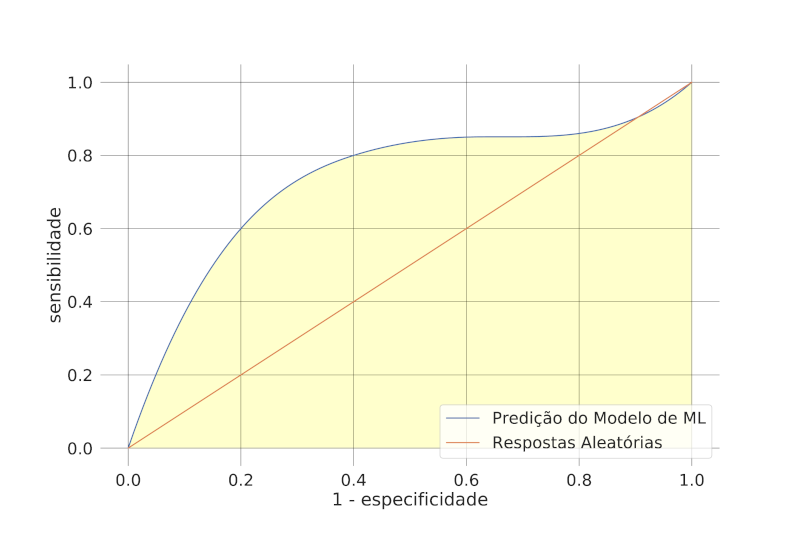
\includegraphics[width=0.85\textwidth]{FIGURES/fig_8.png}
    \caption{Exemplo da curva ROC e AUC (destacada em amarelo). Fonte: Elaborada pelo autor.}
    \label{fig:8}
\end{figure}

Outras métricas estatísticas também podem ser utilizadas, tais como t-\textit{Student} ou valor-\textit{p}, conforme \citet{bib:livroML} e \citet{bib:livroKubat}. Todavia, com menor probabilidade de uso. Dessa forma, apenas as métricas apresentadas acima são consideradas ao longo desta tese e, em particular, as métricas \textit{F1-Score} e AUC, por apresentarem maior confiabilidade nos resultados verdadeiramente válidos.
